\documentclass[xcolor=dvipsnames]{beamer}

\usepackage{graphicx}
\usepackage{bera}% optional: just to have a nice mono-spaced font
\usepackage{listings}
\usepackage{xcolor}
\usepackage{hyperref}


\setbeamertemplate{navigation symbols}{}
\useoutertheme{infolines}
\usecolortheme[named=violet]{structure}
\setbeamertemplate{items}[circle]
\title[cowbells]{The Cowbells Simulation}
\institute[BNL]
{
  Physics Department
  
  \includegraphics[height=1.5cm]{bnl-logo}
}
\author{Brett Viren}
\date{\today}

\DeclareGraphicsExtensions{.pdf,.png,.jpg}
\definecolor{rootpink}{RGB}{255,0,255}

% http://tex.stackexchange.com/questions/83085/how-to-improve-listings-display-of-json-files
\colorlet{punct}{red!60!black}
\definecolor{background}{HTML}{EEEEEE}
\definecolor{delim}{RGB}{20,105,176}
\colorlet{numb}{magenta!60!black}

\lstset{%
  emphstyle=\color{red},
  keywordstyle=\color{black}\bfseries,
    basicstyle=\footnotesize\ttfamily,
    backgroundcolor=\color{background},
    frame=lines,
  identifierstyle=\color{DarkOrchid}\ttfamily,
  commentstyle=\color{Brown}\ttfamily,
  stringstyle=\color{blue}\ttfamily,
  showstringspaces=false}


\lstdefinelanguage{json}{
    basicstyle=\normalfont\ttfamily,
%    numbers=left,
    numberstyle=\scriptsize,
    stepnumber=1,
    numbersep=8pt,
    showstringspaces=false,
    breaklines=true,
    frame=lines,
    backgroundcolor=\color{background},
    literate=
     *{0}{{{\color{numb}0}}}{1}
      {1}{{{\color{numb}1}}}{1}
      {2}{{{\color{numb}2}}}{1}
      {3}{{{\color{numb}3}}}{1}
      {4}{{{\color{numb}4}}}{1}
      {5}{{{\color{numb}5}}}{1}
      {6}{{{\color{numb}6}}}{1}
      {7}{{{\color{numb}7}}}{1}
      {8}{{{\color{numb}8}}}{1}
      {9}{{{\color{numb}9}}}{1}
      {:}{{{\color{punct}{:}}}}{1}
      {,}{{{\color{punct}{,}}}}{1}
      {\{}{{{\color{delim}{\{}}}}{1}
      {\}}{{{\color{delim}{\}}}}}{1}
      {[}{{{\color{delim}{[}}}}{1}
      {]}{{{\color{delim}{]}}}}{1},
}


\begin{document}



\begin{frame}
\titlepage
\end{frame}

\begin{frame}
  \frametitle{Outline}

  \tableofcontents
\end{frame}

\section{Overview}

\begin{frame}
  \frametitle{Overview}
  
  Cowbells is:
  \begin{itemize}
  \item A Geant4 + ROOT application for simulation of particles through materials and detectors.
  \item Flexible in terms of geometry description and simulated data production.
  \item Used to simulate the detectors and beam and cosmic-$\mu$ experiments for BNL WbLS R\&D
  \end{itemize}

  Name comes in a tortured fashion from: 

  \begin{center}
    \textbf{CO}smic-$\mu$ \textbf{W}ater-\textbf{B}ased \textbf{LL}iquid \textbf{S}cintilator.
  \end{center}
  
  \begin{center}
    \url{https://github.com/brettviren/cowbells}
  \end{center}

\end{frame}

\section{Installation}

\begin{frame}[fragile]
  \frametitle{Installation}
  To install cowbells:

  \begin{lstlisting}[langauge=sh]
$ git clone https://github.com/brettviren/cowbells.git
$ mkdir build
$ cd build
$ cmake [-D...] ../cowbells
$ make
  \end{lstlisting}
%$

  You will need to install and tell CMake where to find the various
  dependencies.  See the \href{https://github.com/brettviren/cowbells/blob/master/README.org}{README.org} file in the source for
  more details.

\end{frame}

\section{Running}

\begin{frame}[fragile]
  \frametitle{Running the simulation}

The simulation runs from the command line:

\begin{lstlisting}[language=sh]
$ cowbells.exe --help
Usage: cowbells [options] [configuration files] [Geant4 .mac files]

Options:
  --help                      Print usages and exit
  --output, -o <outputfile>   Set output filename
  --modulies, -m <modules>    Set output modules as comma separated list
  --interface, -u <interface> Set the user interface
  --kinematics, -k <kindesc>  Set the kinematics descriptor
  --physics, -p <physics,list>Set the physics list
  --nevents, -n <#events>     Set the number of events to generate
  --seed, -s <seed>           Seed the random number generator
\end{lstlisting}
%$

Most command line options can also be specified in the configuration file(s).
\end{frame}

\section{Configuration}

\begin{frame}
  \frametitle{Configuration overview}
  \begin{itemize}
  \item Entire configuration may be captured into file(s).
  \item Command line flags may override select configuration items.
  \item Configuration files usually generated via Python (which may use higher-level configuration files)
  \end{itemize}

  Configuration files are in JSON format:
  \begin{itemize}
  \item Simple, text based format from JavaScript
  \item Parsed by \texttt{jsoncpp} (copy included with cowbells)
  \item Resulting data structure interpreted by cowbells
  \end{itemize}

\end{frame}

\begin{frame}
  \frametitle{Major configuration sections}
  \begin{description}
  \item[physics] Physics list
  \item[kinematics] Initial particle kinematics description
  \item[elements] Atomic elements
  \item[materials] Compound materials
  \item[optical] Bulk optical properties of a material.
  \item[shapes] Volume primitives, (shape + dimension)
  \item[volumes] Logical volumes, (shape+material)
  \item[placements] Placed (``physical'') volumes
  \item[surfaces] Optical surface description
  \item[sensitive] Description of sensitive detector
  \end{description}

\end{frame}

\section{Physics List}

\begin{frame}[fragile]
  \frametitle{Physics List}
  
  The physics to implement is handled by the \texttt{Cowbells::PhysicsList} class and can take a combination of these options:

  \begin{description}
  \item[\texttt{em}] Electro-magnetic physics 
  \item[\texttt{op}] Optical processes
  \item[\texttt{had}] Hadronic interaction
  \end{description}

  Command line:
  \begin{lstlisting}[language=sh]
$ cowbells.exe -p em,op    
  \end{lstlisting}
%$ 

Configuration file:
\begin{lstlisting}[language=json,firstnumber=1]
{"physics": 
  { "list": ["em","op"] } }  
\end{lstlisting}
\end{frame}

\section{Kinematics}

\begin{frame}[fragile]
  \frametitle{Kinematics}
  \begin{itemize}
  \item Multiple types of kinematics implemented in C++
  \item Type-specific parameters.
  \item Concise URL-style description for command line
  \end{itemize}

  \begin{lstlisting}[language=sh]
$ cowbells.exe --kinematics \
 'kin://beam?vertex=0,0,0&name=proton&direction=1,0,0&energy=500'
  \end{lstlisting}
%$

  \begin{lstlisting}[language=json]
    "kinematics" : {
        "type" : "gun",
        "count" : 1,
        "particle": "proton",
        "vertex": [0.0, 0.0, 0.0],
        "direction": [1.0, 0.0, 0.0],
        "energy": "500*MeV"
    },
  \end{lstlisting}

\end{frame}

\section{Geometry}

\begin{frame}
  \frametitle{Geometry Configuration}

  Ultimately, you must provide a JSON file by any means necessary.
  Cowbells provides some Python modules to assist in generating one.
  \begin{itemize}
  \item Assure proper JSON format and expected schema.
  \item Python classes associated to JSON configuration items.
  \item Many default elements, materials, and optical properties provided.
  \item Allows for proper handling of units.
  \item A ``builder'' mini-framework for writing detector description generators.
  \end{itemize}
\end{frame}

\begin{frame}
  \frametitle{Example Geometry Generator}
  \begin{itemize}
  \item Main program: \texttt{cowbells/share/gentubdet.py --help}
  \item Simple single-PMT ``tub detector''
  \item Set sample and wall materials and Teflon color.
  \end{itemize}
  Other examples in the \texttt{share/} directory.
\end{frame}

\begin{frame}[fragile]
  \frametitle{Visualization}

  Using HepRApp file:
  \begin{lstlisting}
/vis/open HepRepFile 
/vis/drawVolume
/vis/scene/add/axes            0 0 0 100 mm
/vis/viewer/flush
/vis/scene/add/axes            0 0 0 100 mm
/vis/scene/add/trajectories rich
/vis/modeling/trajectories/create/drawByParticleID
/vis/modeling/trajectories/drawByParticleID-0/set e- blue
/vis/modeling/trajectories/drawByParticleID-0/set e+ cyan
/vis/modeling/trajectories/drawByParticleID-0/set proton red
/vis/modeling/trajectories/drawByParticleID-0/set neutron green
/vis/modeling/trajectories/drawByParticleID-0/set opticalphoton white
/run/beamOn 1
  \end{lstlisting}
  \begin{itemize}
  \item Other Geant4 methods should be possible but not tested.
  \item Todo: convert JSON $\to$ ROOT \texttt{TGeo} objects
  \end{itemize}
\end{frame}

\begin{frame}[fragile]
  \frametitle{Example Visualization: Tub Detector}

  \vspace{-5mm}

  \begin{center}
    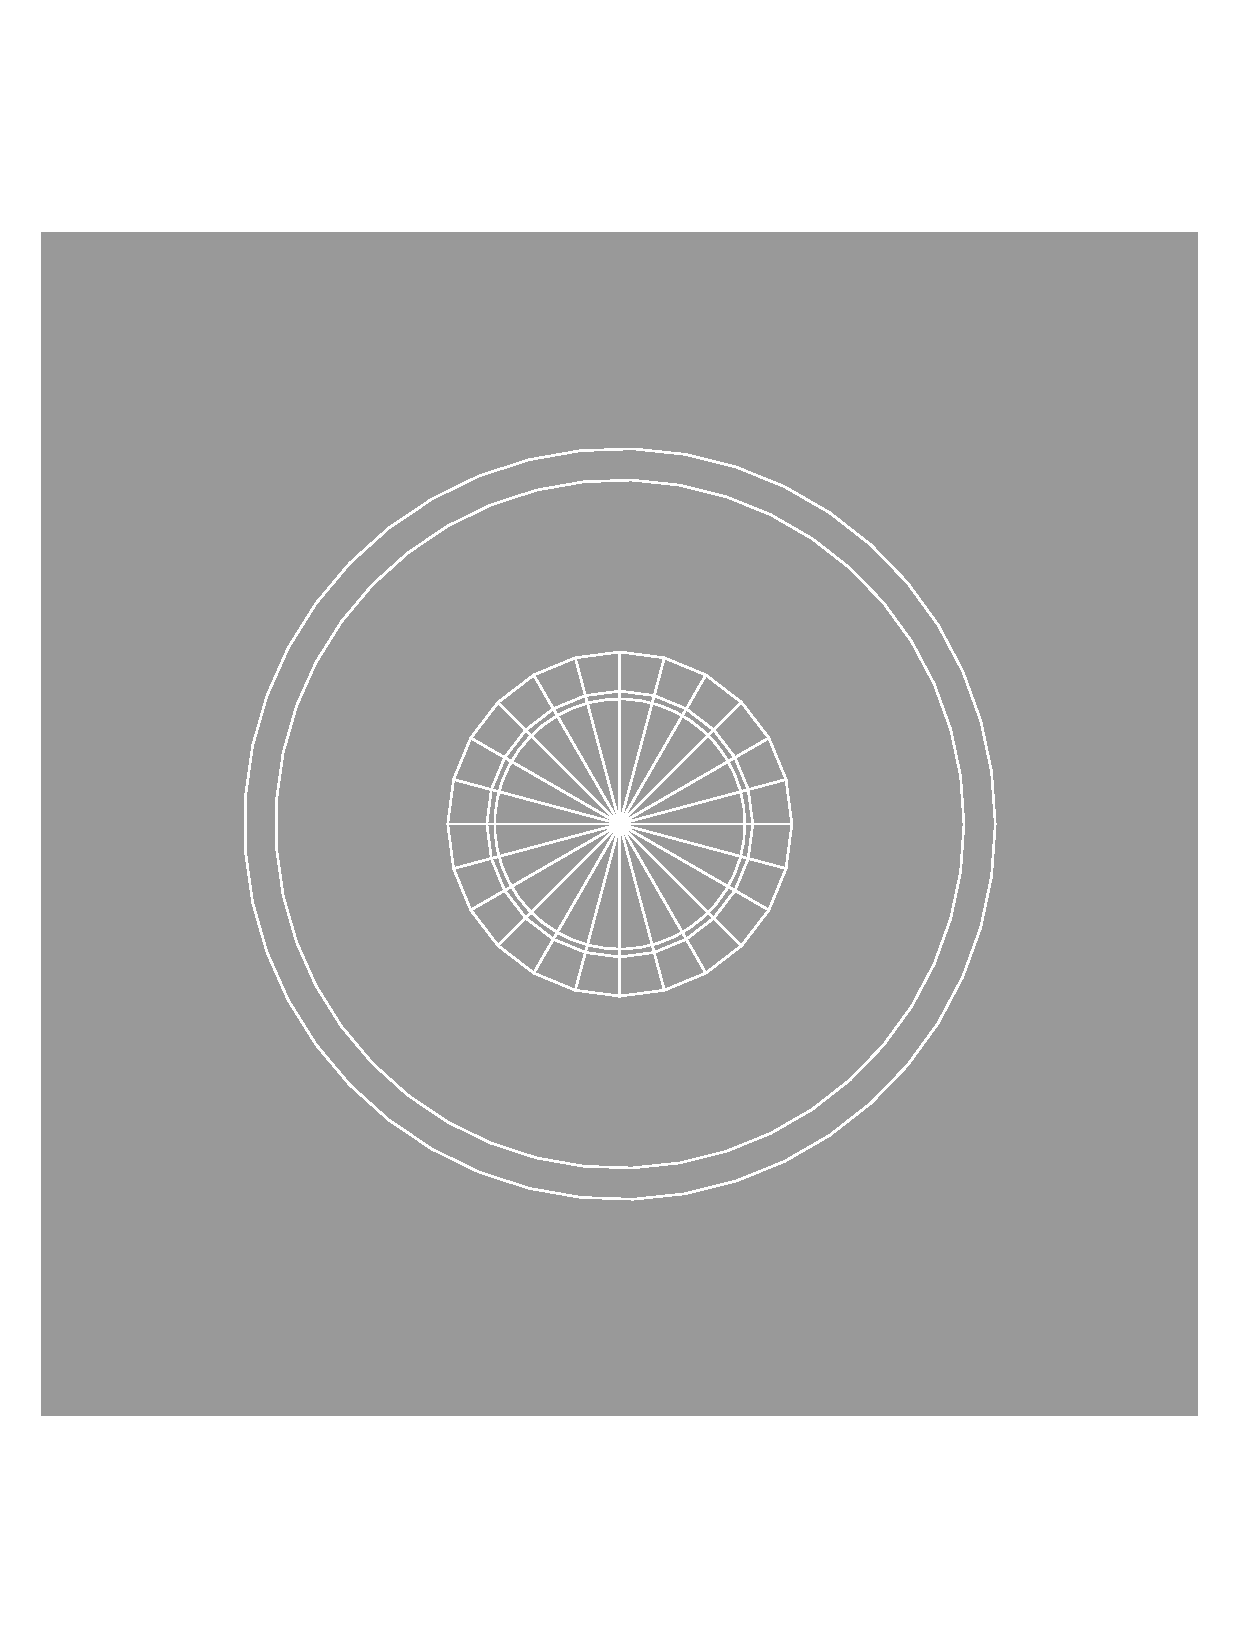
\includegraphics[width=0.3\textwidth]{tubdet-top}
    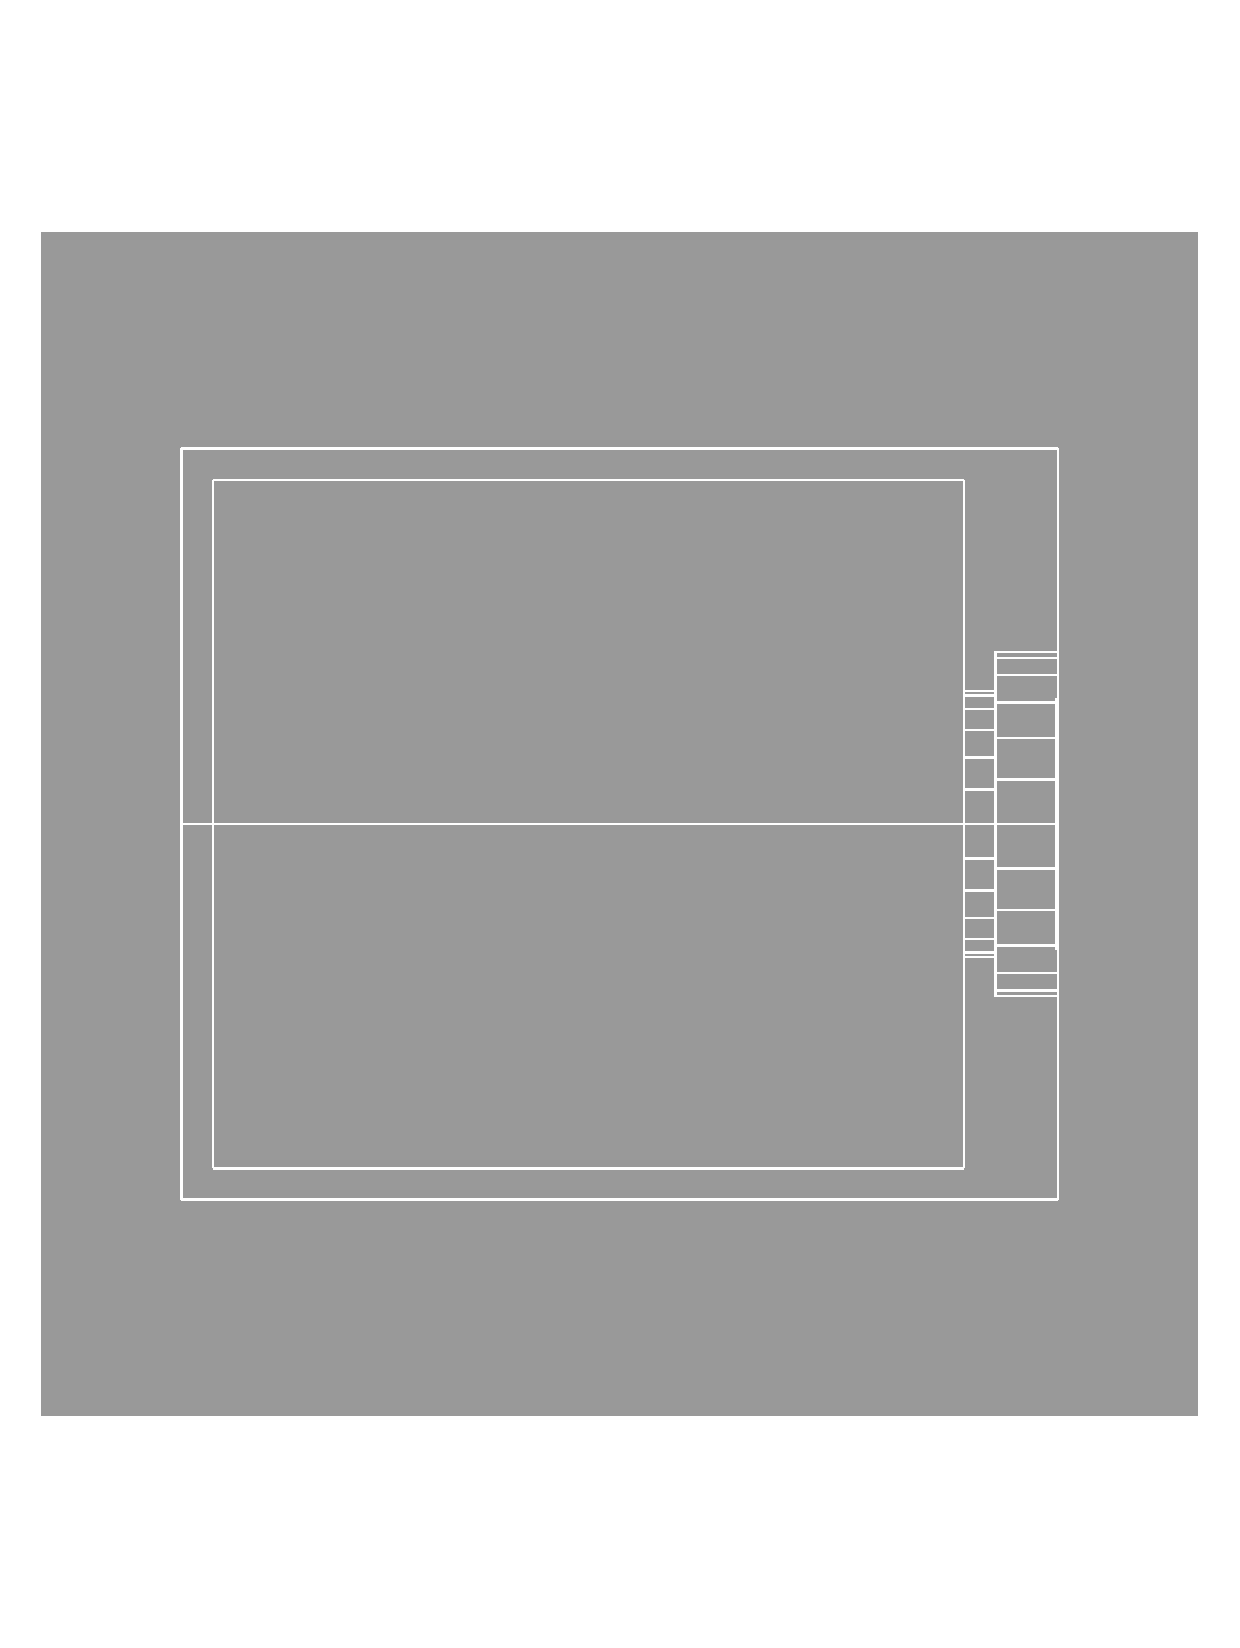
\includegraphics[width=0.3\textwidth]{tubdet-side}
    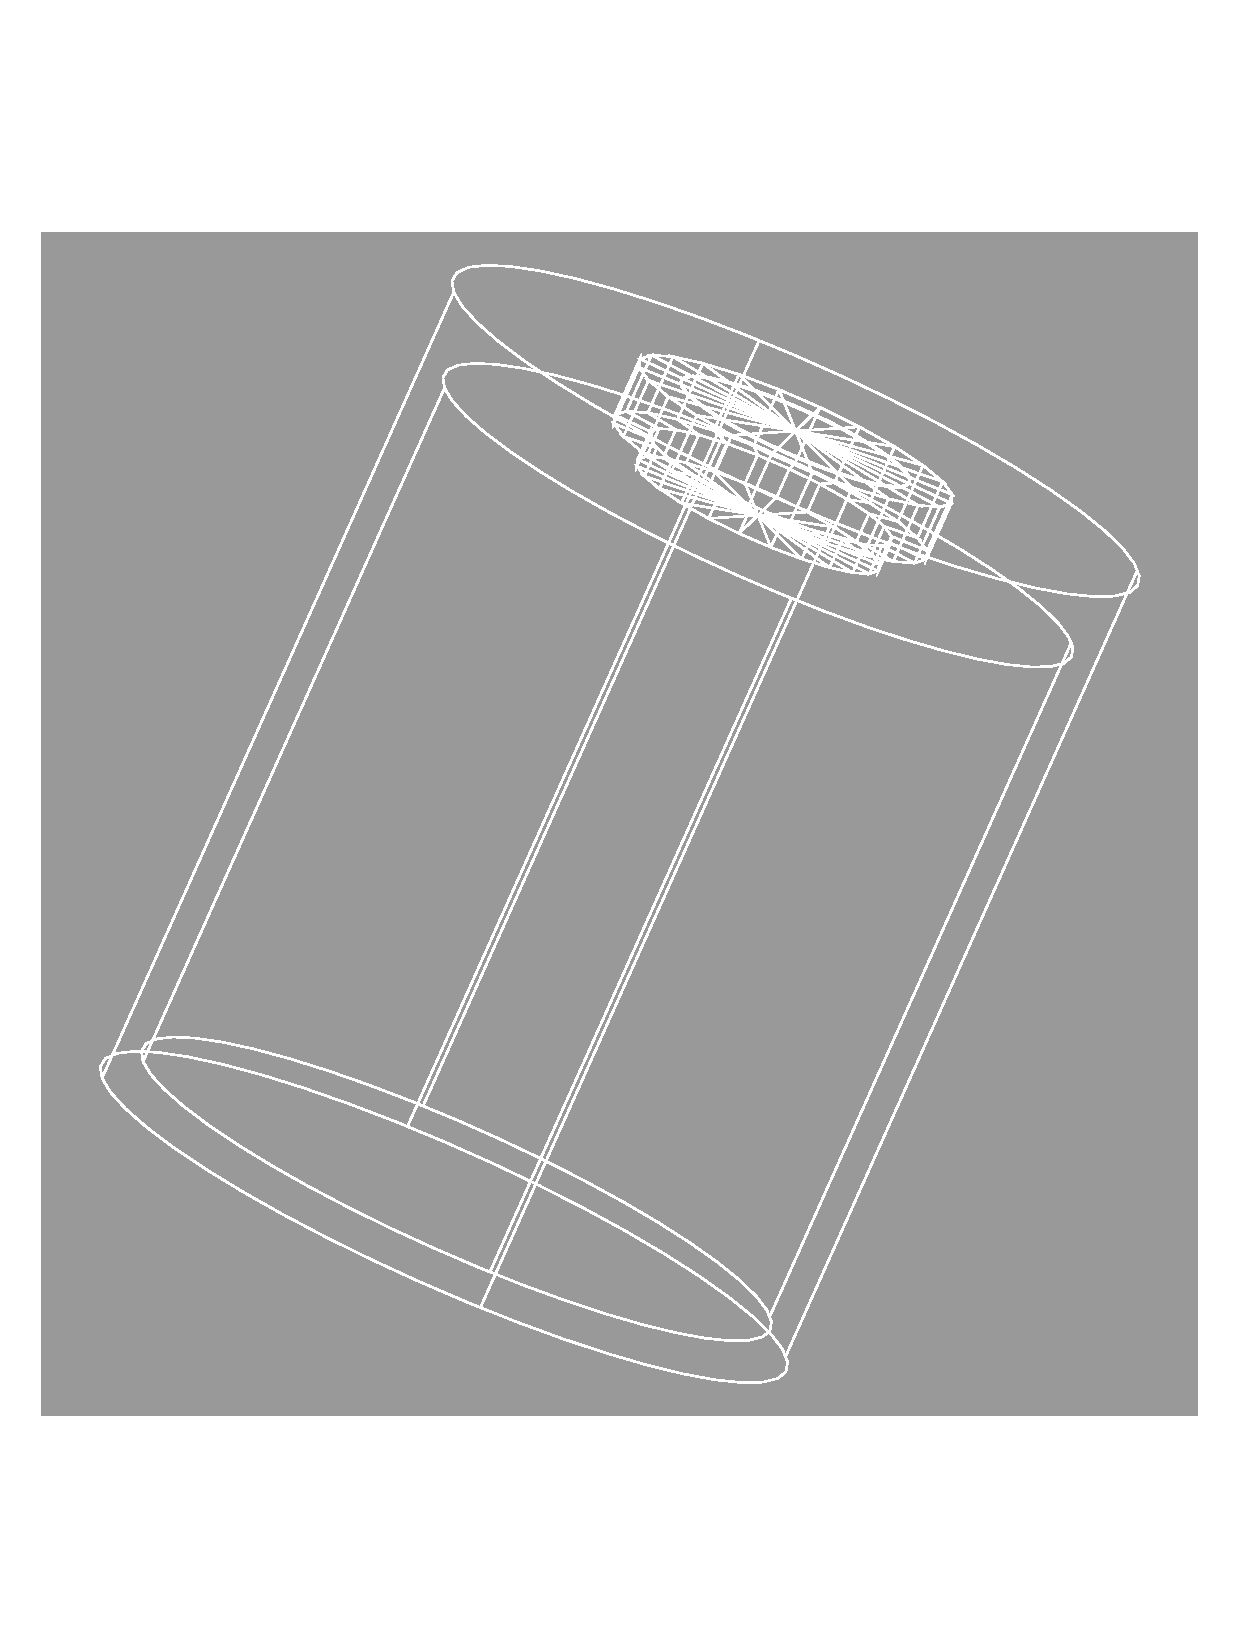
\includegraphics[width=0.3\textwidth]{tubdet-iso}
  \end{center}

  \vspace{-5mm}

  \begin{center}
    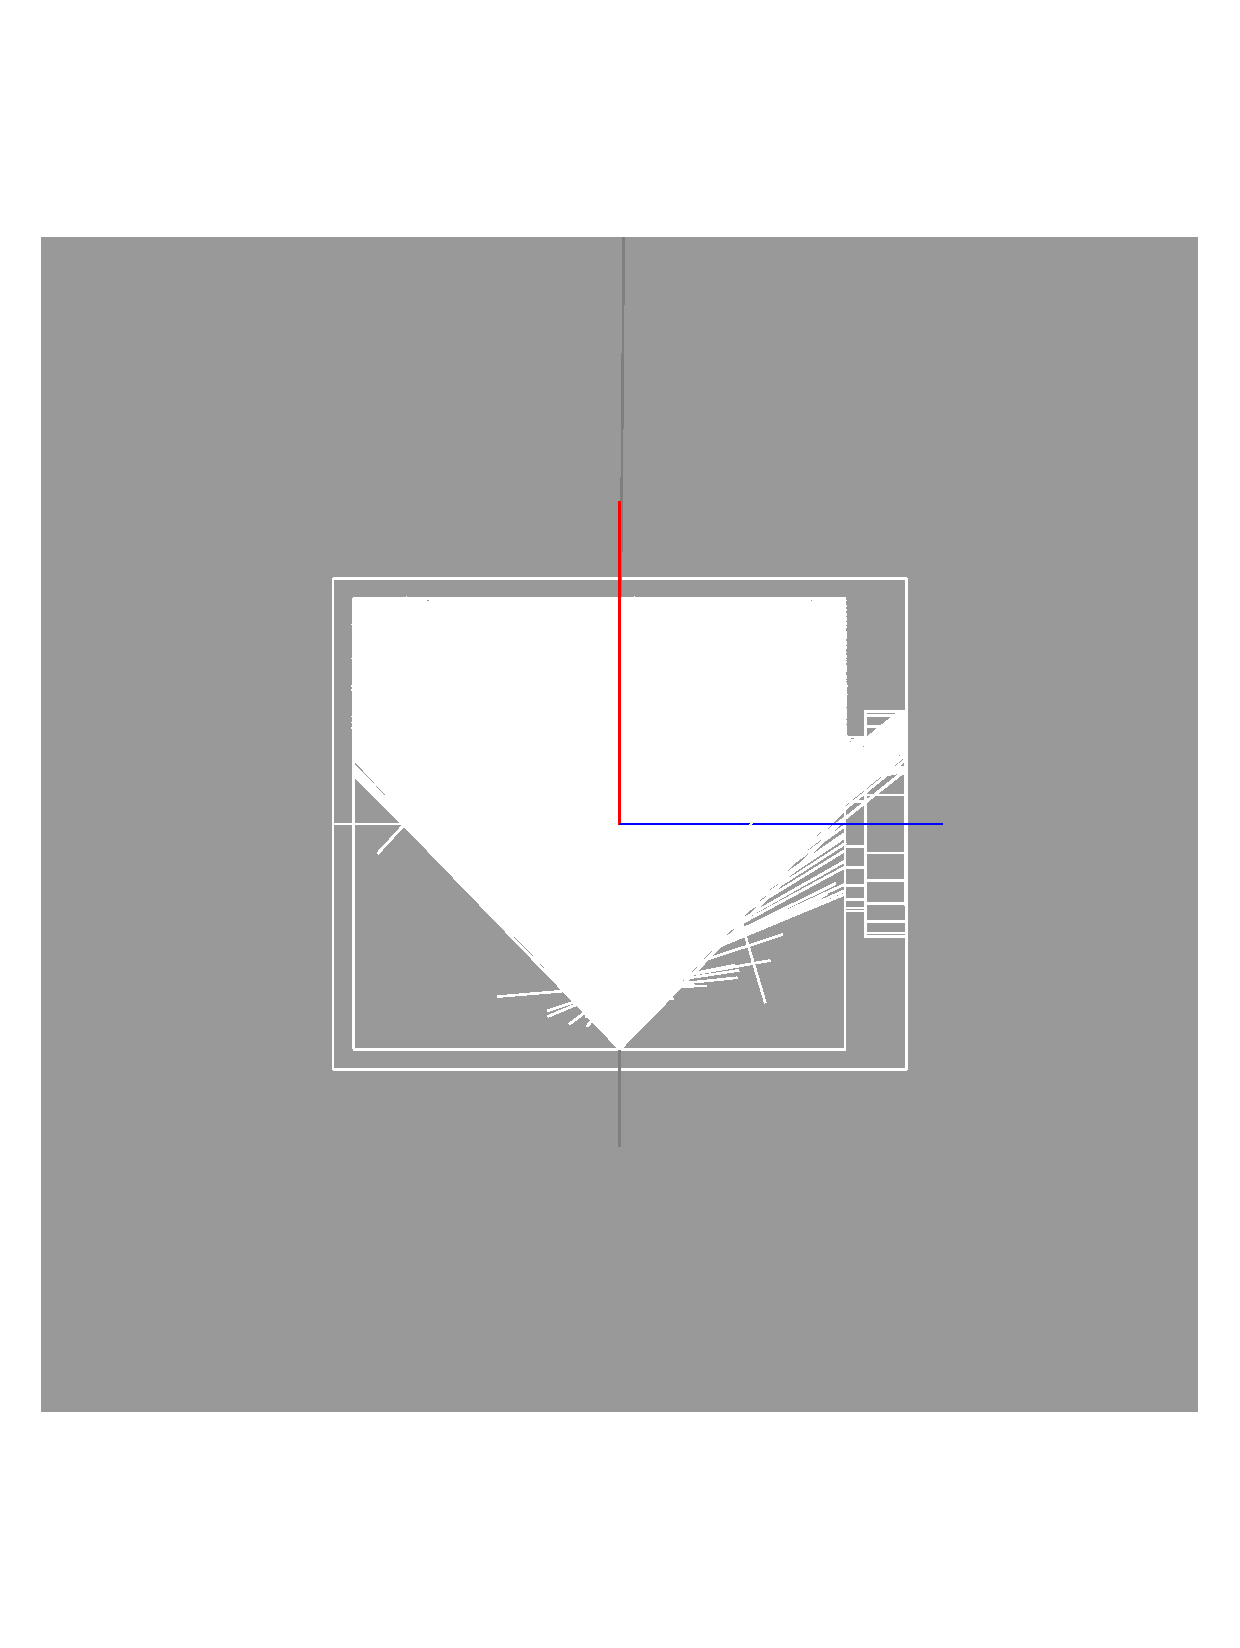
\includegraphics[width=0.3\textwidth,clip,trim=3cm 8cm 3cm 8cm]{mu+-1gev-water-side}
    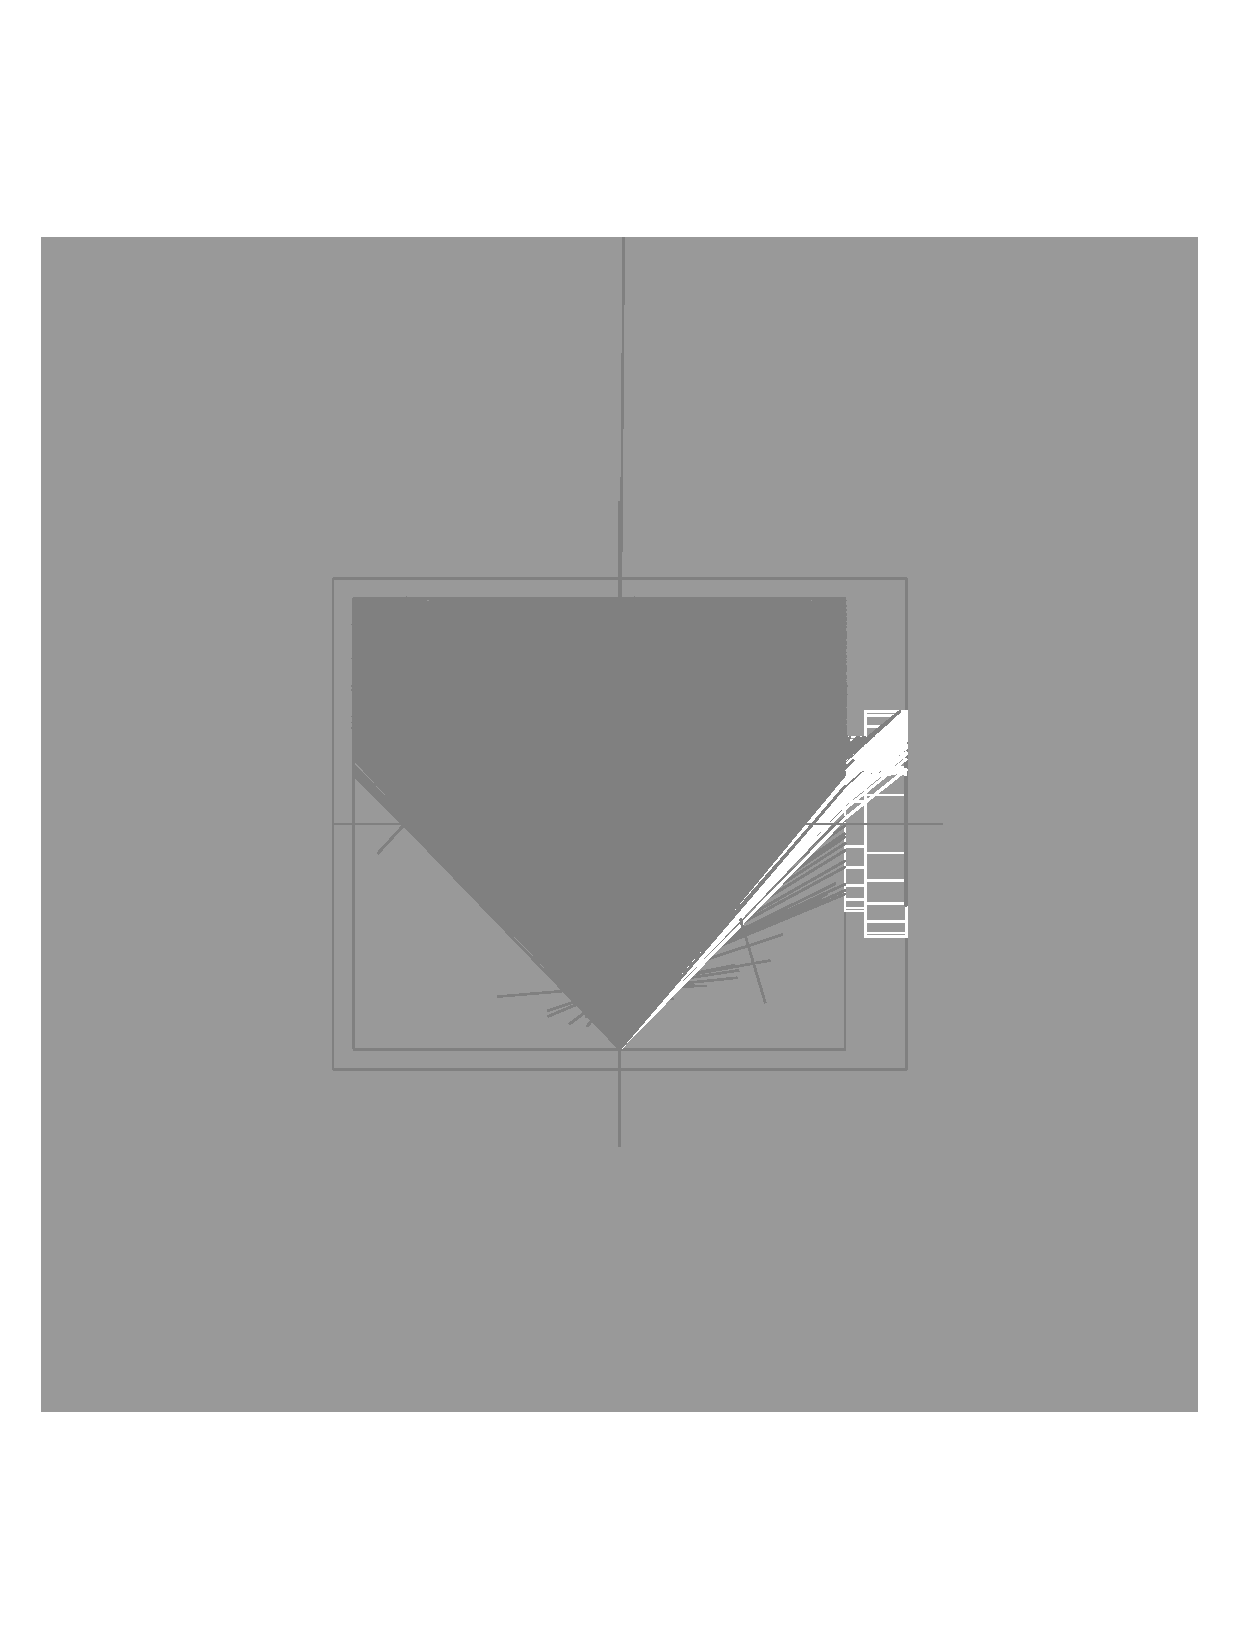
\includegraphics[width=0.3\textwidth,clip,trim=3cm 8cm 3cm 8cm]{mu+-1gev-water-side2}
    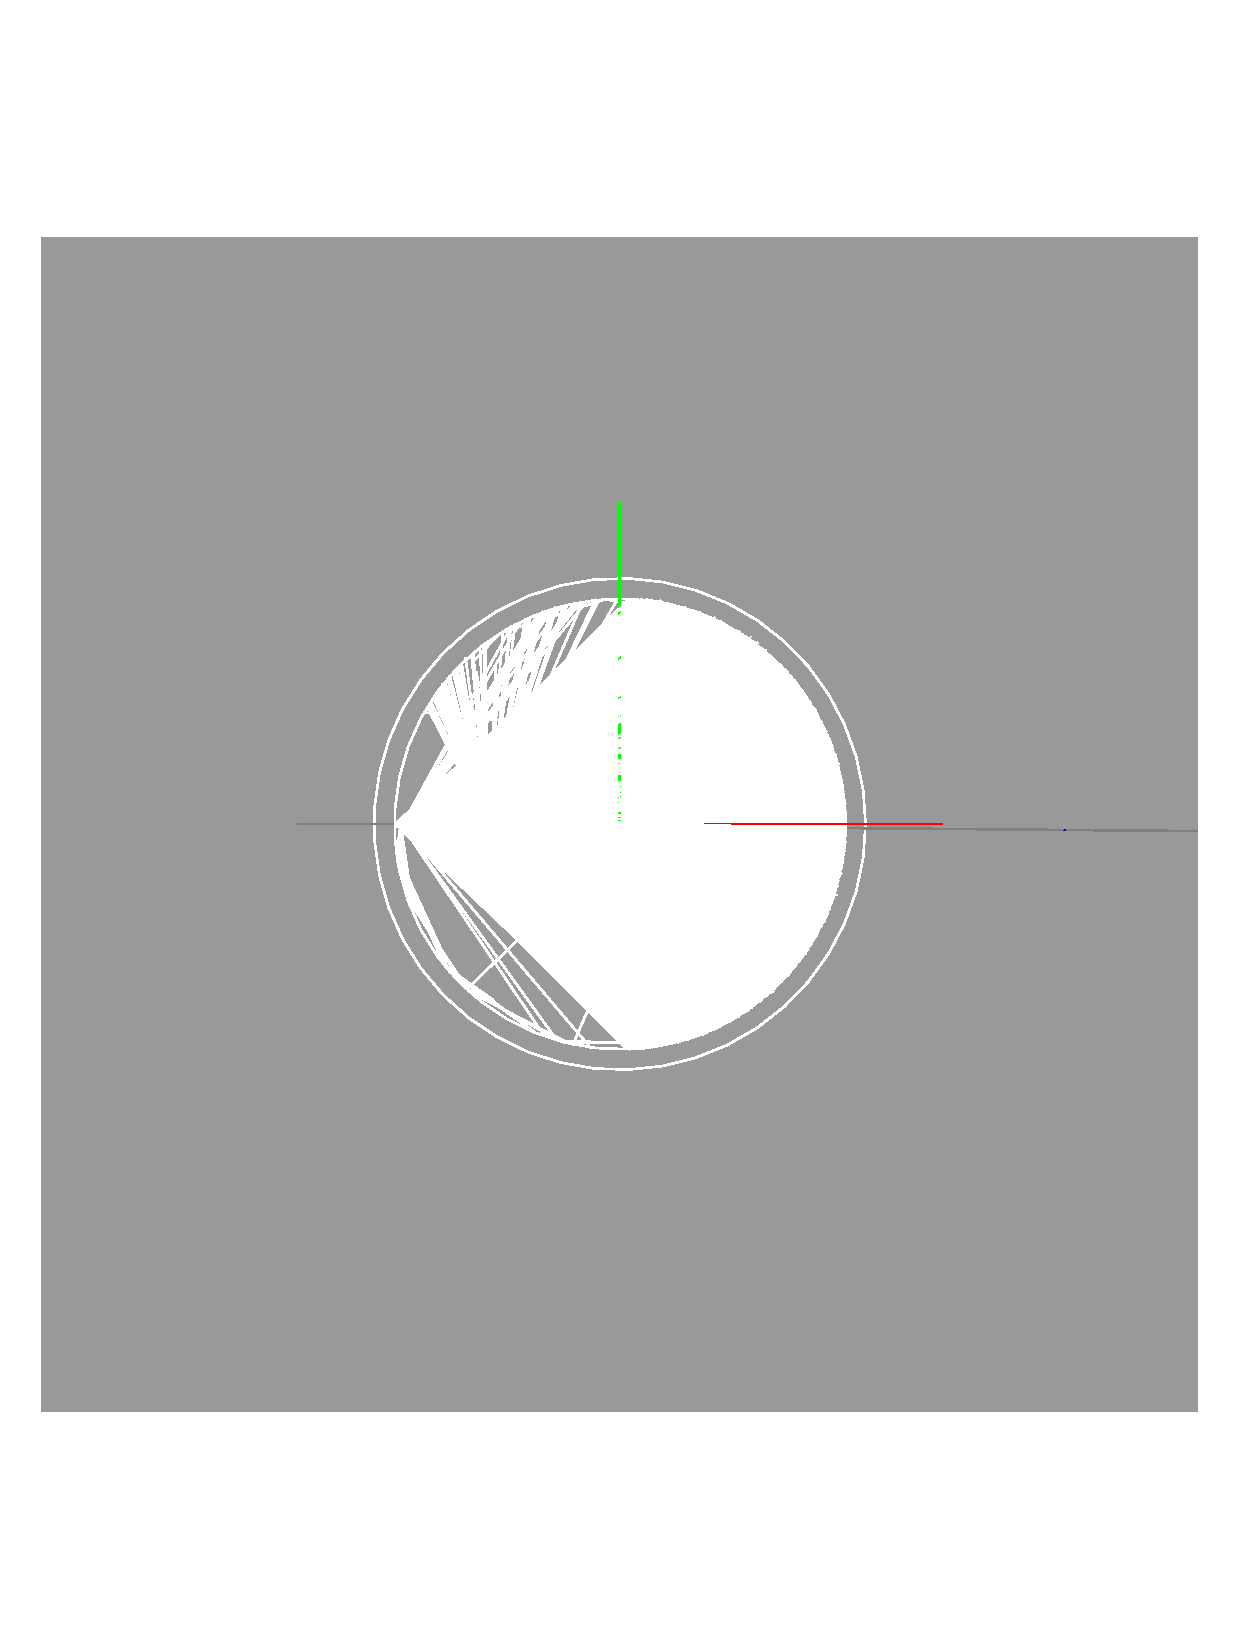
\includegraphics[width=0.3\textwidth,clip,trim=3cm 8cm 3cm 8cm]{mu+-1gev-water-top-internal-reflection2}
  \end{center}

\end{frame}

\begin{frame}[fragile]
  \frametitle{Sensitive Detectors}
  A sensitive detector (eg, a PMT):
  \begin{itemize}
  \item turns an energy deposition (``hit'') into a readout signal in Geant4.
  \item requires Geant4 C++ code and integration with cowbells
  \item multiple types may exist, distinguished by name
  \item multiple instances may exist distinguished by ``touchable'' path
  \item description must match geometry
  \end{itemize}

  \begin{columns}
    \begin{column}{0.5\linewidth}
  \begin{lstlisting}[language=json, basicstyle=\tiny\ttfamily]
  "sensitive": 
  [ 
    {
      "hcname": "TCBialkaliPhotoCathode_HC", 
      "touchables": [
        "pvWorld:0/pvTCBialkaliPhotoCathode:1", 
        "pvWorld:0/pvTCBialkaliPhotoCathode:2"
      ], 
      "logvol": "lvTCBialkaliPhotoCathode", 
      "world_pv": "pvWorld", 
      "name": "TCBialkaliPhotoCathode_SD"
    }, 
  \end{lstlisting}
    \end{column}
    \begin{column}{0.5\linewidth}
  \begin{lstlisting}[language=json, basicstyle=\tiny\ttfamily]
    { 
      "hcname": "MagicBialkaliPhotoCathode_HC", 
      "touchables": [
        "pvWorld:0/pvMagicWaterSample:0/pvMagicWindowA:0/pvMagicBialkaliPhotoCathode:0", 
        "pvWorld:0/pvMagicWaterSample:0/pvMagicWindowB:0/pvMagicBialkaliPhotoCathode:0"
      ], 
      "logvol": "lvMagicBialkaliPhotoCathode", 
      "world_pv": "pvWorld", 
      "name": "MagicBialkaliPhotoCathode_SD"
    } ], 
  \end{lstlisting}
      
    \end{column}
  \end{columns}

\end{frame}

\section{Output}

\begin{frame}
  \frametitle{Output Data from Cowbells}
  \begin{itemize}
  \item ROOT tree branched by a single \texttt{Cowbells::Event} object
  \item \texttt{Event} holds several \texttt{std::vector}'s
  \item Vectors fill based on ``output modules'' activated:
    \begin{description}
    \item[\texttt{kine}] initial 4-pos/mom, PDG ID
    \item[\texttt{hits}] volume, hit collection names, PDG, E, pos
    \item[\texttt{steps}] track, parent, PDG, mass, e-dep, pos, dt
    \item[\texttt{stacks}] track, parent, \#photons (scint/ceren)
    \end{description}
  \end{itemize}
\end{frame}


\end{document}